\section{Building Convolutional Neural Network with Keras}
\label{sec:buildcnn}
%
As we discussed in the last section (\ref{subsec:introduction_keras}), Keras 
has a series of layers that were specifically created to support convolutional 
neural networks.
By definition, a fully connected layer connects every neuron in the layer and 
at the first layer it's connected to all the inputs. 
And all these connections create a problem known as the curse of 
dimensionality. 
That is, the more neurons and connections we have, the more weights we must 
train. 
This issue appears often, it is one of reasons why deep neural networks can 
take a long time to learn. 
To understand this issue a bit more, let's consider the case of working with 
images. 
Assume that we have an 8 megapixel image and that we want to learn 
something from this image. 
To do that, we construct a network with a dense layer. 
Since every pixel in the image can contain unique data, they each contribute 
uniquely to determining the logic resulting from analysing the image. 
Therefore we need to connect each pixel to each neuron in our first layer. 
Let's say that we have 1000 neurons in the first dense layer.
We have to connect the data from each pixel to each neuron so we end up with 
1000 neurons connected to 8 million pixel values, with each connection having 
its own weight that needs to be trained. 
That works out to 8 billion weights we have to train. 
And with most images it's even more. In a color image, each pixel has three 
colors. 
One for red, green, and blue channels of the image. 
So there are actually 24 billion weights to train.
Solving this explosion in the number of weights we have to train is one of the 
key reasons convolutional neural networks were developed. 
%
\subsection{How works CNNs}
\label{ssec:cnnworks}
%
Convolutional neural network address our two concerns of working with image 
type data namely, many weights to train and being able to detect objects based 
on their general appearance rather than precisely matching an image. 
A lot of research has been performed when working with images and has 
resulted in subtle layers that you find in almost all convolutional neural 
networks. 
And these are the convolution layers you find in Keras. 
To understand the function of these layers, let's go over the structure of a 
convolutional neural network, which classifies objects and images.
%
Let's walk through this diagram so we can get an overview of how convolutional 
neural networks work and how we implement them using Keras. 
We see the image data is passed through the convolutional layer, then through 
a non-linear ReLU activation and then to a pool layer. 
And then to a second convolution with ReLU layer and a second pool layer. 
Finally, to a fully connected layer and then to a second fully connected 
layer for classification. 
So we can divide our convolutional neural network into four operations. 
Convolution, non-linearity, you see via ReLU, pooling, and classification. 
You will find these four operations in almost all convolutional neural networks. 
Let's look at each operation in detail so we understand how to set parameters 
and pass data when we construct our convolutional neural network in Keras.
Convolutional neural networks are the current state-of-art architecture for
image classification. They are used in practice today in facial recognition, self
driving cars, and detecting whether an object is a hot-dog.
%
\subsection{Convolution}
\label{ssec:convolution}
%
A convolution consists of a kernel, shows in figure \ref{fig:convolution}, 
(green square above), also called filter,
that is applied in a sliding window fashion to extract features from the input.
This filter is shifted after each operation across the input by an amount called
strides. At each operation, a matrix multiply of the kernel and current region
of input is calculated. Filters can be stacked to create high-dimensional
representations of the input.
%
\begin{figure}[!h]
\centering
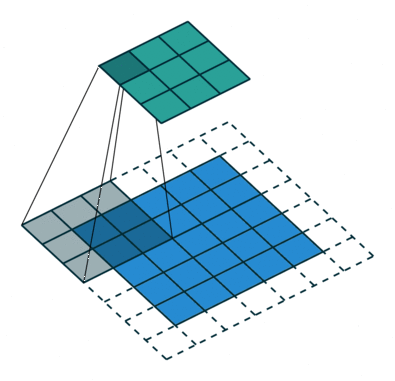
\includegraphics[width=\linewidth]{conv_arithmetic}
\caption{Convolution operation to extract features from the input}
\label{fig:convolution}
\end{figure}
%
There are two ways of handling differing filter size and input size, namely
same padding and valid padding.
Same padding will pad the input border with zeros (as seen above) to ensure the
input width and height are preserved. Valid padding does not pad.
Typically, you will want to use same padding or you will rapidly reduce the
dimensionality of your input.
Finally, an activation function (typically a ReLU\footnote{In the context of 
artificial neural networks, the rectifier is an activation function defined as 
the positive part of its argument:\\ \(f(x) = x^{+} = \text{max}(0,x)\)}), 
represented in figure \ref{fig:relu}, is applied to give the convolution non-linearity.
ReLU’s are a bit different from other activation functions, such as sigmoid or
tanh, as ReLUs are one-sided.
This one-sided property allows the network to create sparse representation
(zero value for hidden units), increasing computational efficiency.
%
\begin{figure}[htb]
\centering
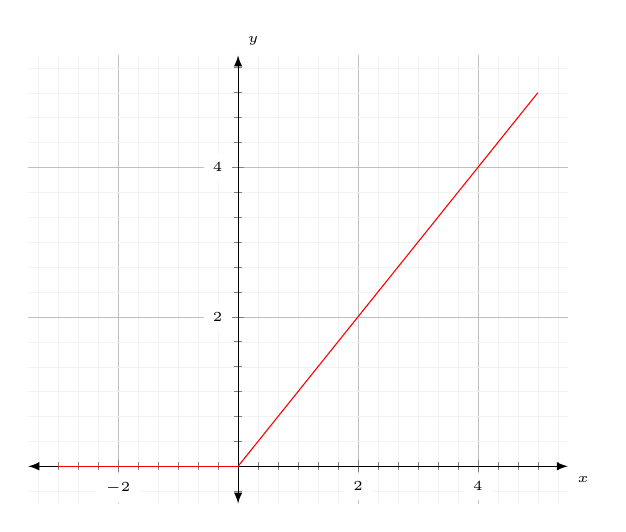
\begin{tikzpicture}
    \begin{axis}[
        domain=-3:5,
        grid=both,
    	grid style={line width=.1pt, draw=gray!10},
    	major grid style={line width=.2pt,draw=gray!50},
    	axis lines=middle,
    	minor tick num=5,
    	enlargelimits={abs=0.5},
    	axis line style={latex-latex},
    	ticklabel style={font=\tiny,fill=white},
    	xlabel style={at={(ticklabel* cs:1)},anchor=north west},
    	ylabel style={at={(ticklabel* cs:1)},anchor=south west},
    	xlabel={\tiny $x$},
    	ylabel={\tiny $y$}
    ]
        \addplot+[mark=none,red,domain=-3:0] {0};
        \addplot+[mark=none,red,domain=0:5] {x};
    \end{axis}
\end{tikzpicture}
\caption{Rectified linear unit (\textbf{ReLU})\\ \(F(x) = x^{+} = \text{max}(0,x)\)}
\label{fig:relu}
\end{figure}
%
\subsection{Pooling}
\label{ssec:pooling}
Pooling is an operation to reduce dimensionality. 
It applies a function summarizing neighbouring information.
Two common functions are max pooling and average pooling.
By calculating the max of an input region, the output summarizes intensity of
surrounding values.
Pooling layers also have a kernel and padding, and are moved in strides, as 
represented in figure \ref{fig:pooling}.
To calculate the output size of a pooling operation, you can use the formula:
\begin{equation}
 \text{Input Width} - \text{kernel width} + 2 * \text{padding}  / \text{strides} + 1
\end{equation}
%
\begin{figure}[htb]
\centering
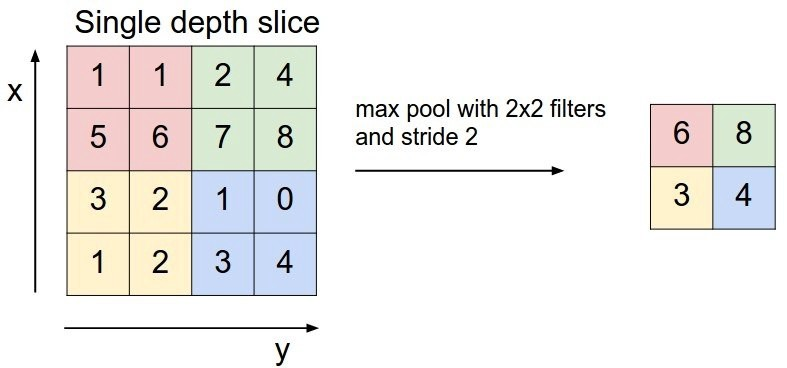
\includegraphics[width=\linewidth]{pooling}
\caption{Max pooling is the application of a moving window across a 2D input 
space, where the maximum value within that window is the output}
\label{fig:pooling}
\end{figure}
%
\subsection{Fully Connected Layer}
\label{ssec:fully_connected}
Fully connected layers you are likely familiar with from neural networks.
Each neuron in the input is connected to each neuron in the output;
fully-connected.
Due to this connectivity, each neuron in the output will be used at most one
time.
%
\begin{equation}
  \sum_{i=1}^{n} \,  x \, \cdot \, W+b
\end{equation}
%
\begin{figure}[htb]
\centering
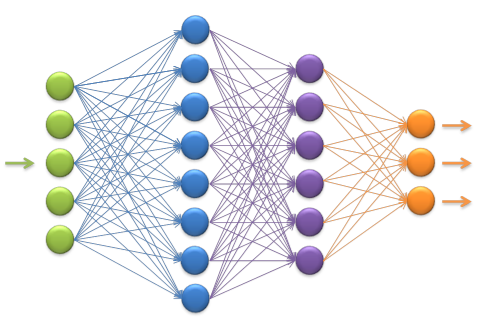
\includegraphics[width=\linewidth]{fully_connected}
\caption{Deep neural networks layers}
\label{fig:fully_connected}
\end{figure}
%
\\\noindent In a CNN, the input is fed from the pooling layer into the fully connected layer.
Depending on the task, a regression or classification algorithm can be applied
to create the desired output, a representative example is shown in figure \ref{fig:fully_connected}.
